\documentclass[11pt, oneside]{article} 
\usepackage{geometry}
\geometry{letterpaper} 
\usepackage{graphicx}
	
\usepackage{amssymb}
\usepackage{amsmath}
\usepackage{parskip}
\usepackage{color}
\usepackage{hyperref}

\graphicspath{{/Users/telliott_admin/Tex/png/}}
% \begin{center} 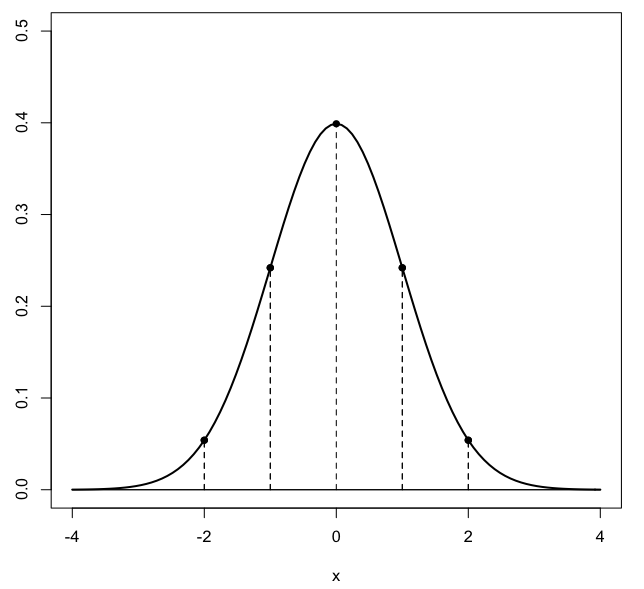
\includegraphics [scale=0.4] {gauss3.png} \end{center}

\title{Kepler Summary}
\date{}

\begin{document}
\maketitle
\Large

In this Chapter we finish up our treatment of Kepler and the orbits of the planets.  The first part is Kepler's Third Law (K3).

\[ T^2 = \frac{(2 \pi)^2}{GM} \ a^3 \]

where $T$ is the period, $GM$ is our constant from before, and $a$ is the length of the half-major axis of the ellipse.  In other words, the period of an orbit is the $3/2$ power of the "radius", technically the semi-major axis of the ellipse.

This formula is pretty easy to derive for a circular orbit (see the chapter on orbital velocity).  The problem here is that the velocity is not constant and the orbit is an ellipse.  Luckily we have a simple formula for the area of an ellipse.

Start with K2 (Varberg's version, where $\ddot{A} = 0$):
\[ 2 \ \frac{dA}{dt} =  h \]

Integrate with respect to time over one revolution obtaining an ellipse with area $\pi a b$ and period $T$
\[ 2 \pi a b = hT \]
\[ T^2 = (\frac{2 \pi a b}{h})^2 \]
Now, go back to the equation for the orbit
\[ r(1 + e \cos \theta) = \frac{h^2}{GM} \]
For simplicity, let $k = h^2/GM$ so
\[ r(1 + e \cos \theta) = k  \]
\[ r = \frac{k}{1 + e \cos \theta}  \]

Consider one-half an orbit between $\theta = 0 \rightarrow \theta = \pi$.  At the start, $\theta = 0$ so
\[ r = \frac{k}{(1 + e)}  \]
at the end $\theta = \pi$ and
\[ r = \frac{k}{(1 - e)}  \]

Recall that this $r$ was really $\mathbf{r} \cdot \mathbf{u_r}$.  As a signed distance the latter is really minus.  So subtracting the former from the latter we get the distance between them is $-a -a = -2a$ and
\[ -2a = -  \frac{k}{(1 - e)} -  \frac{k}{(1 + e)} \]
\[ 2a = \frac{k}{(1 - e)} + \frac{k}{(1 + e)} \]
\[ a = \frac{k}{(1 - e^2)} \]

If you're uncomfortable with this, go back to the chapter on the polar form of the ellipse, we had 
\[ r(1 + e \cos \theta) = ep = a(1 - e^2) \]
Since $ep = k$, we have the same thing.

For an ellipse 
\[ 1 - e^2 = \frac{a^2 - c^2}{a^2} = \frac{b^2}{a^2} \]
so
\[ \frac{b^2}{a^2} = \frac{k}{a} \]
\[  b^2 = ka \]

We had 
\[ T^2 = (\frac{2 \pi a b}{h})^2 \]
substituting for $b^2$
\[ T^2 = (\frac{2 \pi a}{h})^2 \ ka \]
and substituting for $k$
\[ = (\frac{2 \pi a }{h})^2 \  \frac{ah^2}{GM}  \]
\[ = \frac{(2 \pi)^2}{GM} \ a^3 \]
which is K3.  

$GM$ is the gravitational constant times the mass of the sun.  The term due to the angular momentum $h$ has dropped out.

Note that we can get an estimate for $GM$ from observation of the orbits of the planets, and that $G$ can be determined very simply, allowing us to find $M$, and "weigh the sun".

\section*{Summary of K1}

\subsection*{unit vectors and velocity}
The position vector (from the sun to the planet) is $\mathbf{r}$.  Starting from our definition of the unit vector in the $\mathbf{r}$ direction as
\[ \mathbf{u_r} = \ \langle \cos \theta, \sin \theta \rangle \]
where $\theta$ is the angle with the positive $x$-axis, we find $\mathbf{u_{\theta}} \perp \mathbf{u_r}$
\[ \mathbf{u_{\theta}} = \ \langle -\sin \theta, \cos \theta \rangle \]
and confirm orthognality
\[ \mathbf{u_r} \cdot \mathbf{u_{\theta}} = 0 \]
Remembering that $\theta = \theta(t)$, we easily obtain by the chain rule
\[ \dot{\mathbf{u}}_\mathbf{r} = \dot{\theta} \mathbf{u_{\theta}} \]
\[  \dot{\mathbf{u}}_\mathbf{\theta} = -\dot{\theta} \mathbf{u_{r}} \]
$r$ is the magnitude of $\mathbf{r}$
\[ \mathbf{r} = r \mathbf{u_r} \]
The velocity $\mathbf{v}$
\[ \mathbf{v} = \dot{\mathbf{r}} = \dot{r} \mathbf{u_r} + r \dot{\mathbf{u}}_\mathbf{r}  =  \dot{r} \mathbf{u_r} +  r \dot{\theta}  \mathbf{u_{\theta}}\]
We use a vector identity that is easy to prove
\[ \frac{d}{dt} \ (\mathbf{a} \times \mathbf{b}) = \dot{\mathbf{a}} \times \mathbf{b} + \mathbf{a} \times \dot{\mathbf{b}} \]
to calculate with Feynman's "dots"
\[ \frac{d}{dt} \ (\mathbf{r} \times \mathbf{v}) \]
\[ =  \frac{d}{dt} \ (\mathbf{r} \times \dot{\mathbf{r}}) \]
\[  =  \dot{\mathbf{r}} \times \dot{\mathbf{r}} +  \mathbf{r} \times \ddot{\mathbf{r}} = 0\]
because any vector's cross-product with itself is zero (including minus itself), which is true for the second term involving the acceleration.
\subsection*{acceleration}
An actual expression for the acceleration is just a matter of working through the dots
\[ \mathbf{a} = \dot{\mathbf{v}} = \ddot{\mathbf{r}} = \frac{d}{dt} \ (\dot{r}\mathbf{u_r} + r \dot{\theta} \mathbf{u_{\theta}}) \]
 \[ = \ddot{r}\mathbf{u_r} + \dot{r}\dot{\mathbf{u}}_\mathbf{r} + \dot{r} \dot{\theta} \mathbf{u_{\theta}} + r \ddot{\theta} \mathbf{u_{\theta}} + r \dot{\theta}  \dot{\mathbf{u}}_\mathbf{\theta}\]
substituting for $\dot{\mathbf{u}}_\mathbf{r}$ and $\dot{\mathbf{u}}_\mathbf{\theta}$ from above
\[ = \ddot{r}\mathbf{u_r} + \dot{r}\dot{\theta} \mathbf{u_{\theta}} + \dot{r} \dot{\theta} \mathbf{u_{\theta}} + r \ddot{\theta} \mathbf{u_{\theta}} - r \dot{\theta}^2  \mathbf{u}_\mathbf{r}\]
\[ = (\ddot{r} - r \dot{\theta}^2)  \mathbf{u}_\mathbf{r} + (2\dot{r} \dot{\theta} + r \ddot{\theta}) \mathbf{u_{\theta}}  \]
Rewrite the coefficient for $\mathbf{u_{\theta}}$ as
\[  \frac{1}{r}(2r \dot{r} \dot{\theta} + r^2\ddot{\theta}) = \frac{1}{r} \frac{d}{dt} (r^2\dot{\theta})  \]
\subsection*{angular momentum}
We find that the acceleration $\mathbf{a} = \dot{\mathbf{v}}$ has two parts of which the second (in $\mathbf{u_{\theta}}$)
\[ \frac{1}{r} \ \frac{d}{dt} \ r^2 \dot{\theta} = 0 \]
 is zero because $\mathbf{a}$ is all radial.  Hence $r^2 \dot{\theta} = h$ where $h$ is a constant.  Multiplied by the mass $m$, $mh$ becomes the conserved quantity, angular momentum.  It is also twice the area "swept out" and this is the statement of K2.

We get the vector $\mathbf{h}$ by defining the plane of motion as the $xy$-plane ($\mathbf{u_r} \times \mathbf{u_{\theta}} = \hat{\mathbf{k}}$) and
\[ \mathbf{h} = \mathbf{r} \times \mathbf{v} = r \mathbf{u_r} \times (\dot{r} \mathbf{u_r} +  r \dot{\theta}  \mathbf{u_{\theta}}) \]
the first term is zero so
\[ = r^2  \dot{\theta} ( \mathbf{u_r} \times \mathbf{u_{\theta}} ) = r^2  \dot{\theta}  \ \hat{\mathbf{k}} \]

\subsection*{key step}

With these preliminary steps we come to the key part of the derivation.  I like Varberg's version best.  The radial acceleration is
\[ \mathbf{a} = -\frac{GM}{r^2} \mathbf{u_r} \]
Compute $\mathbf{a} \times \hat{\mathbf{k}}$ (recall that $\mathbf{a}$ is in the $-\mathbf{u_r}$ direction) by recognizing that $-\mathbf{u_r} \times \hat{\mathbf{k}} = \mathbf{u_{\theta}}$ so
\[ \mathbf{a} \times \hat{\mathbf{k}} = \frac{GM}{r^2} \mathbf{u_{\theta}} \]
but from above $\dot{\mathbf{u}}_\mathbf{r} = \dot{\theta} \mathbf{u_{\theta}}$ so we have the crucial substitution:
\[ \mathbf{a} \times \hat{\mathbf{k}} = \frac{GM}{r^2 \dot{\theta} } \dot{\mathbf{u}}_\mathbf{r} \]
\[ \mathbf{a} \times \hat{\mathbf{k}} = \frac{GM}{h} \dot{\mathbf{u}}_\mathbf{r} \]
Now we just integrate with respect to time and get
\[ \int \mathbf{a} \times \hat{\mathbf{k}} = \int \frac{GM}{h} \dot{\mathbf{u}}_\mathbf{r}  \]
\[ \mathbf{v} \times \hat{\mathbf{k}} = \frac{GM}{h} \mathbf{u}_\mathbf{r} + \mathbf{d} \]
where $\mathbf{d}$ is a constant \emph{vector} of integration.
One last trick, we dot with $\mathbf{r}$ and simplify the left-hand side dramatically
\[ \mathbf{r} \cdot ( \mathbf{v} \times \hat{\mathbf{k}}) = (\mathbf{r} \times \mathbf{v}) \cdot  \hat{\mathbf{k}} = \mathbf{h} \cdot \hat{\mathbf{k}} = h \]
So
\[ h = \mathbf{r} \cdot (\frac{GM}{h} \mathbf{u}_\mathbf{r} + \mathbf{d}) \]
\[ \frac{h^2}{GM} = \mathbf{r} \cdot (\mathbf{u}_\mathbf{r} + \frac{h}{GM} \mathbf{d} ) \]
Define $k = h^2/GM$ and $e = hd/GM$ and $\theta$ as the angle between the constant vector $\mathbf{d}$ and $\mathbf{u}_\mathbf{r}$, so finally
\[ k = r (1 + e \cos \theta) \]

which for $e < 1$ is an ellipse.

\end{document}  